\section{Introduction}

As most practitioners in the domain of data management systems are discovering, One Size doesn't Fit All~\cite{Stonebraker-2007}. Today most production data management systems are following something similar to a fractured mirrors approach~\cite{Ramamurthy-2002}.  Primary OLTP data-stores take user facing writes and some reads, while other specialized systems serve complex queries or accelerate query results through caching.  
The most common data systems found in these architectures include relational databases, NoSQL data stores, caching engines, search indexes and graph query engines. This specialization has in turn made it critical to have a reliable and scalable data pipeline that can capture these changes happening for primary source-of-truth systems and route them through the rest of the complex data eco-system. 

%LinkedIn's data architecture consists of Oracle and MySQL as source-of-truth primary database technologies. There are a large number of specialized systems that have been built for serving complex use-cases like graph queries, search queries and ranking entities. Since reads outnumber writes by a large fraction in our workload, in many cases, we prefer to serve reads out of replica data stores; a technique commonly referred to as read-scaling. For example, there are cases when a single Oracle (running on expensive hardware) is the primary data store while many MySQL or Oracle instances (running on cheaper hardware) are serving reads. 
%There are also other use-cases in the company that involve query result pre-computation, caching and near-line stream processing. 
%There is therefore a need to capture all the changes that are happening to the primary databases and process it to populate the secondary data stores and indexes.
%We also want to have a common data format that is both shared by all consumers and is independent of the source of truth. 

There are two families of solutions that are typically used for building such a pipeline.

\begin{itemize}
\item\emph{Application-driven Dual Writes}: In this model, the application layer writes to the database and in parallel, writes to another messaging system. This looks simple to implement since the application code writing to the database is under our control. However it introduces a consistency problem because without a complex coordination protocol (e.g.~Paxos~\cite{paxos} or ~2-Phase~Commit~\cite{Gray-1978}) it is hard to ensure that both the database and the messaging system are in complete lock step with each other in the face of failures. Both systems need to process exactly the same writes and need to serialize them in exactly the same order. Things get even more complex if the writes are conditional or have partial update semantics. 
\item\emph{Database Log Mining}: In this model, we make the database the single source-of-truth and extract changes from its transaction or commit log. This solves our consistency issue, but is practically hard to implement because databases like Oracle and MySQL (the primary data stores in use at LinkedIn) have transaction log formats and replication solutions that are proprietary and not guaranteed to have stable on-disk or on-the-wire representations across version upgrades. Since we want to process the data changes with application code and then write to secondary data stores, we need the replication system to be user-space and source-agnostic. This independence from the data source is especially important in fast-moving technology companies, because it avoids technology lock-in and tie-in to binary formats throughout the application stack.
\end{itemize}

After evaluating the pros and cons of the two approaches, we decided to pursue the ``log mining'' option, prioritizing consistency and ``single source of truth'' over ease of implementation. 

%% Comments from Lin
%% The paragraph below needs a crisp list of strength/differentiators databus provides. Organize points in bullets will help.
%% Then we can have list of use cases, the longer, the more angels, the better.
  
In this paper, we introduce Databus, LinkedIn's Change Data Capture pipeline, which supports Oracle and MySQL sources and a wide range of downstream applications. 
The Social Graph Index which serves all graph queries at LinkedIn, the People Search Index that powers all searches for members at LinkedIn and the various read replicas for our Member Profile data are all fed and kept consistent via Databus. 
In the rest of the paper, we focus on Databus' unique architectural features:
\begin{itemize}
\item{Pull-model}
\item{Externally-clocked}
\item{Consumption from arbitrary point in the change stream}
\item{Isolation between sources and consumers: both in terms of performance and the specifics of the implementations}
\end{itemize}

While building Databus, we have encountered some practical design and implementation issues which we also cover in this paper. 
In particular, we discuss implementation details and performance measurements around:
\begin{itemize}
\item{Event definition, serialization and portability}
\item{Minimizing load on the data source}
\item{Filter push-down and partitioned consumption}
\item{Achievements in scalability, high-availability and low latency}
\end{itemize}

%There are custom adaptors written for Oracle and MySQL which extract the changes happening in the database and convert them to a storage-neutral format. 
%It is extremely easy to add support for other kinds of data sources as long as they provide a transaction log with some amount of rewindability.
%These changes are then transported via a lossless tier while retaining the source consistency semantics to the final consumers. 
%Databus allows consumers to fall behind indefinitely and still catchup while shielding the data source from abusive scan queries. 
%The subscription API allows applications to subscribe to changes from one or more data sources, and filter based on the keys of the events.  
\begin{figure}
\centering
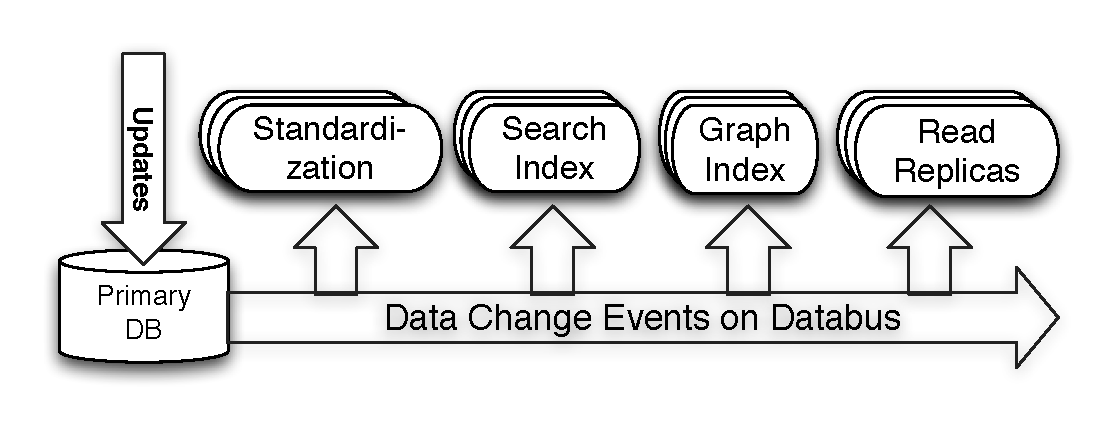
\epsfig{file=figures/databus-use-cases.eps, width=3in}
\caption{LinkedIn: Databus applications}
\label{fig:databus-use-cases}
\end{figure}

The next section dives deeper into the requirements that drove us towards the design and implementation decisions outlined above. 



